%% LaTeX2e class for student theses
%% sections/content.tex
%%
%% Karlsruhe University of Applied Sciences
%% Faculty of  Computer Science and Business Information Systems
%% Distributed Systems (vsys)
%%
%% Prof. Dr. Christian Zirpins
%% christian.zirpins@hs-karlsruhe.de
%%
%%
%% Version 0.2, 2017-11-15
%%
%% --------------------------------------------------------
%% | Derived from sdqthesis by Erik Burger burger@kit.edu |
%% --------------------------------------------------------

\chapter{Implementierung eines ActivityPub Prototyps}
Die IDataSource Implementierung wird für das Unternehmen angefertigt in der die Bachelor Thesis bearbeitet wird. Im Falle man möchte den Service mit einer anderen Datenquelle versorgen, kann das IDataSource Interface implementiert und so angepasst werden, dass eine andere Datenbank Verwendung findet.\\

\begin{figure}[h]
	\begin{minipage}{\textwidth}
		\centering
		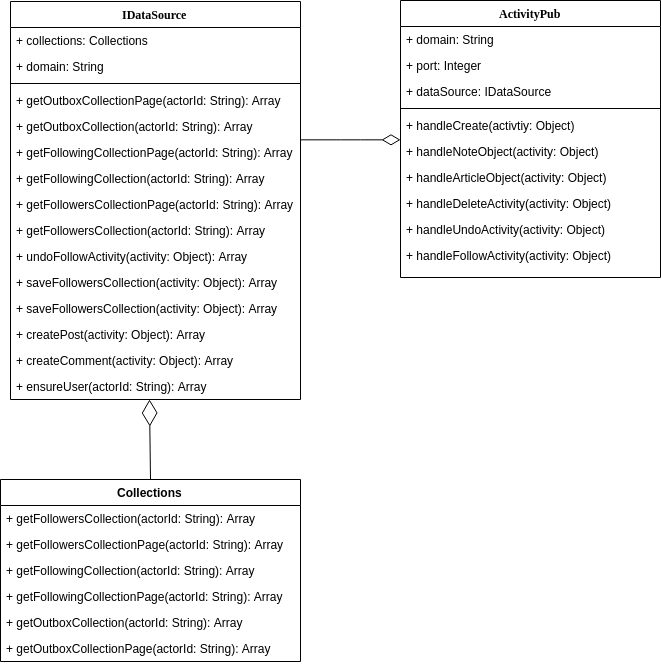
\includegraphics[scale=0.5]{figures/klassendiagramm-activitypub.png}
		\label{klassendiagramm-activitypub}
		\caption{Hauptkomponenten des förderierten Servers}
	\end{minipage}
\end{figure}
\section{Server-zu-Server Protokoll}